\documentclass[10pt]{article}
\usepackage{natbib}
\usepackage{times}
\usepackage[T1]{fontenc}
\usepackage[utf8]{inputenc}
\usepackage[pdftex]{graphicx}
\usepackage{caption}
\captionsetup[figure]{justification=raggedright,labelfont=bf}
\usepackage{fullpage} % 1" margins
\usepackage{setspace}
\setstretch{1.5}
\usepackage{tabu}
%\usepackage{sectsty}
%\sectionfont{\nohang\centering\normalsize\sc}   % capitalize initial letters
%\subsectionfont{\nohang\centering\normalsize\rm\em}

\renewcommand{\thetable}{S\arabic{table}}

% eat the colon so figures are labeled but have blank captions
% \makeatletter
% \renewcommand\fnum@figure[1]{\figurename~\thefigure\ignorespaces}
% \makeatother

%% Article
\begin{document}
\raggedright
\parindent 0.5in


\begin{table}%[tbhp]
  \centering
  \small
  \caption{Global and regional sampling of clades.}
  \begin{tabu} to \textwidth {X[-3,l,b]|X[-1,r,b]X[-1,r,b]X[-1,r,b]|X[-1,r,b]X[-1,r,b]X[-1,r,b]|X[-1,r,b]X[-1,r,b]X[-1,r,b]|X[1,r,b]X[1,r,b]X[1,r,b]}
   \hline
    & \multicolumn{3}{c|}{global} & \multicolumn3{c|}{Hengduan Mountains} & \multicolumn3{c|}{Himalayas-QTP} & \multicolumn3{c}{temperate/boreal East Asia}\\
   clade                                                  & total & sampled & \% & total & sampled & \% & total & sampled & \% & total & sampled & \%  \\
   \hline
   \textit{Acer}                                          & 129   & 118     & 91 & 45    & 29      & 64 & 24    & 15      & 63 & 80    & 72      & 90  \\
   \textit{Allium}                                        & 800   & 378     & 47 & 34    & 29      & 85 & 55    & 37      & 67 & 89    & 100     & 89  \\
   Clematidinae+ Anemoninae                               & 495   & 177     & 36 & 76    & 32      & 42 & 45    & 26      & 58 & 152   & 72      & 47  \\
   Delphineae                                             & 756   & 312     & 41 & 225   & 74      & 33 & 83    & 44      & 53 & 90    & 51      & 57  \\
   \textit{Cyananthus}                                    & 66    & 47      & 71 & 41    & 28      & 68 & 26    & 24      & 92 & 14    & 10      & 71  \\
   \textit{Isodon}                                        & 100   & 63      & 63 & 55    & 40      & 73 & 20    & 9       & 45 & 36    & 24      & 67  \\
   \textit{Ligularia- Cremanthodium- Parasenecio} complex & 380   & 75      & 20 & 152   & 60      & 39 & 62    & 12      & 19 & 148   & 27      & 18  \\
   \textit{Meconopsis}                                    & 54    & 47      & 87 & 25    & 22      & 88 & 36    & 34      & 94 & 2     & 2       & 100 \\
   Microsoroideae                                         & 248   & 147     & 59 & 45    & 42      & 93 & 38    & 35      & 92 & 80    & 66      & 83  \\
   Pinaceae                                               & 234   & 226     & 97 & 34    & 32      & 94 & 26    & 24      & 92 & 63    & 63      & 100 \\
   Polygoneae                                             & 663   & 257     & 39 & 92    & 61      & 66 & 85    & 75      & 88 & 160   & 127     & 79  \\
   Primulaceae                                            & 900   & 354     & 39 & 205   & 114     & 56 & 150   & 68      & 45 & 80    & 55      & 69  \\
   \textit{Rhodiola}                                      & 70    & 57      & 81 & 32    & 28      & 88 & 37    & 30      & 81 & 34    & 20      & 59  \\
   \textit{Rhododendron}                                  & 1000  & 351     & 35 & 237   & 120     & 51 & 124   & 42      & 34 & 300   & 105     & 35  \\
   \textit{Rosa}                                          & 175   & 102     & 58 & 49    & 27      & 55 & 29    & 20      & 69 & 64    & 35      & 55  \\
   \textit{Saussurea}                                     & 416   & 147     & 35 & 108   & 73      & 68 & 130   & 63      & 48 & 157   & 56      & 36  \\
   Saxifragaceae+ Grossulariaceae                         & 760   & 313     & 41 & 209   & 54      & 26 & 155   & 45      & 29 & 170   & 102     & 60  \\
   \textit{Thalictrum}                                    & 150   & 104     & 69 & 38    & 34      & 89 & 40    & 25      & 63 & 48    & 32      & 67  \\
   \hline
    
  \end{tabu}
\end{table}

%%% Local Variables: 
%%% mode: latex
%%% TeX-master: "SI"
%%% End: 


\clearpage
\newpage

\section*{Materials and Methods}



\bibliography{bibliography/biblio}
\bibliographystyle{ecol_let}

% \begin{figure}
% \begin{center}
% 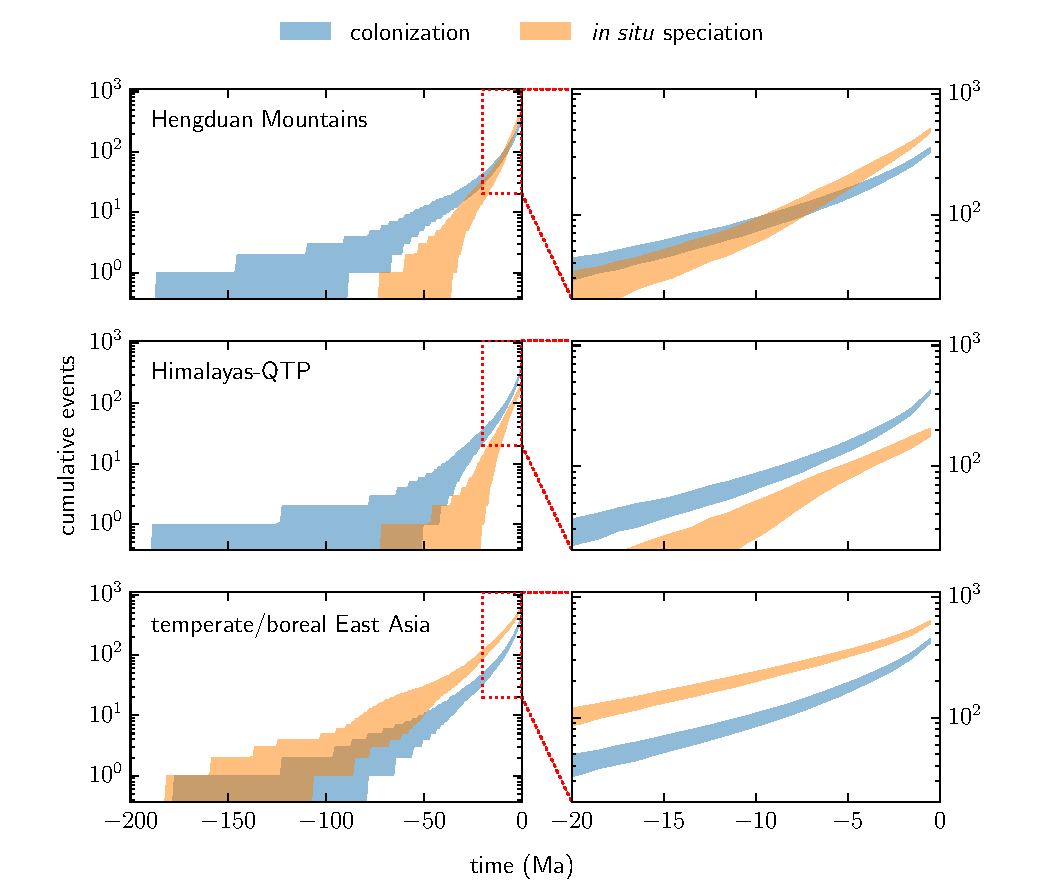
\includegraphics[width=.99\textwidth]{figures/figure_cumulative_events/figure_cumulative_events.pdf}
% \end{center}
% \caption{Assembly of regional floras by colonization and \textit{in situ} speciation events in 18 plant clades, inferred from ancestral-range reconstructions on time-calibrated molecular phylogenies. Shaded regions indicate the 5--95\% quantile intervals for the cumulative number of events through time from 500 pseudoreplicated joint biogeographic histories designed to account for phylogenetic uncertainty (see text). Panels on the right focus on the last 20 Ma, in which differences in regional assembly are most apparent. In the Hengduan Mountains region, cumulative \textit{in situ} speciation overtakes colonization about 8 Ma, whereas for the Himalayas-QTP, colonization remains the dominant process. \textit{In situ} speciation thus appears to have played a disproportionately large role in assembling the Hengduan Mountains flora since the late Miocene compared to the Himalayas-QTP, consistent with the theory of uplift-driven diversification in the Hengduan Mountains region.}
% \label{fig:cumevents}
% \end{figure}

\end{document}

%%% Local Variables:
%%% mode: latex
%%% TeX-master: t
%%% End:
